\documentclass[output=paper]{langscibook}
\ChapterDOI{10.5281/zenodo.4545035}

\author{Felix Hoberg\affiliation{Leipzig University}}
\title[Dialogue-oriented evaluation of MS Skype Translator for Catalan-German]{Dialogue-oriented evaluation of Microsoft's Skype Translator in the language pair Catalan-German} 
\abstract{This paper presents preliminary results of the work on Microsoft's Skype Translator. Tackling the question of how to evaluate such technology on a dialogue-oriented level, a case study on 21 German-speaking participants was conducted. Despite not having any proficiency in Catalan, these participants had to text-chat with Catalan native speakers via Skype, while the Skype Translator was activated. The sessions were observed by means of an eye tracking system. The collected data thus represents a naturalistic starting point to evaluate how users structure computer-mediated communication situations when real-time machine translation is involved and thereby they have to rely on that output.}

\begin{document}
\renewcommand{\lsChapterFooterSize}{\footnotesize}
\SetupAffiliations{mark style=none}
\maketitle

\section{Introduction} 

Automatic language processing, auto speech recognition and machine translation (MT) are considered valuable innovations by the language industry. However, progress in this field is still viewed skeptically, which in turn calls for continuous evaluation of the aforementioned systems \citep[i.e.][]{ramlow_maschinelle_2009, bowker_machine_2019}, especially when it comes to dialogic interactions between humans and MT. Microsoft’s Skype Translator will thus serve as a central element in this case study, as it offers real-time machine translation in 10 languages in voice and video chats and 60 languages in text chats.

To highlight how MT evaluation can be applied to services like the Skype Translator and how it has to be modeled on the dialogue-oriented level, the project combines research in the fields of communication research \citep{beiswenger_sprachhandlungskoordination_2007} and machine translation. Additionally, this project aims to examine the behaviour of conversation's participants when an MT engine is involved \citep{fiser_investigating_2017}.

To achieve these goals, an exploratory eye-tracking-based case study was carried out. In that study, Skype Translator-mediated text chats between German and Catalan native speakers were captured in order to investigate the fixation duration and count on characteristical areas of interest of the Skype Translator. 

This paper thus aims exclusively at giving a first impression on which aspects to analyse in the above mentioned context. For that reason, Section \ref{sec:background} introduces the theoretical background in terms of research on dialogue and conversation in the context of computer-mediated communication. Section \ref{sec:Rdesign} gives insights on the overall project conception, before explaining in detail to which extent the collected data is used for this analysis. Then, Section \ref{sec:Results} presents early findings of the eye tracking data and situates them along the theoretical background, before the conclusion in Section \ref{sec:conclusion} sums up the analysis, going back to the overall project.




%------------------------------------

\section{Background}
\label{sec:background}

\subsection{Research on dialogue and conversation}
\label{subsec:research}
% Computer-mediated Communication

    Since the early 1990s, various concepts in communication research have been modelled and restructured to fit on modern computer-mediated communication \citep[cf.][7]{fiser_investigating_2017}. Apart from taking a look at global concepts such as text, sender, recipient or conversation, the interest in research has now passed on to questions which reflect the transitional processes web-based communication has undergone over the last two decades: How do we interact online? How does online interaction change our ways of communicating? Can we still speak of sender and recipient after all? How do we cope with this great amount of data and the rising machine learning technologies? \citep[cf.][]{beiswenger_sprachhandlungskoordination_2007}.
    
    These questions also implicitly refer to the phenomena of turn-taking and speaker switch or the rising use of the term \textit{hypertext} to describe digital textual behaviour \citep[cf.][]{storrer_sprachliche_2001}, central elements which have already been extensively studied regarding analog, face-to-face and monolingual web-based communication, but so far have not been adopted to bilingual, machine-translated, web-based conversations such as presented in this paper. This gap might be attributed to the fact that online communication follows different rules than offline communication.
    There are two obvious differences between oral, face-to-face and chat communication. The latter appears in written or typed form and lacks of mostly all the non- and paraverbal elements like gesture, intonation or eye contact etc. which usually help to structure the communication act \citep[cf.][172]{beiswenger_sprachhandlungskoordination_2007}.
    
    In contrast, an online chat message passes through more sections between a sender and an addressee than an oral, face-to-face talk. From the sender's mind, it goes from typing on the keyboard to the computer's short-term memory and from there to the server the software in use is connected to. From that server it goes to the addressee's software and it is subsequently processed by the computer to be displayed on screen before the addressee can spend cognitive resources on it \citep[cf.][146]{beisswenger_empirische_2017}. In the case of the Skype Translator, one additionally has to take into account the time it takes to send, machine-translate and receive the original message. In the case of high latency, this time gap can have a severe impact on communication -- while the person on the receiving end is still answering one incoming message, the other may already have sent another text. This can result in an asynchronous communication.
    
    Thus, the use of computer-mediated communication technology, and in this case, to be precise, the Skype Translator, leads to a change in the communication process of sending and receiving messages. A text chat message has to be completely written before it can be sent\footnote{Real-time text chat, where the text is transmitted immediately so that every user can observe the production process, will not be considered here.} and it has to be received and read before it can be reacted to. At the same time, apart from in oral communication, the communication partners are not necessarily in the same location, nor near at all (cf. ibid.: 146). 
    
    \citet[cf.][3]{storrer_sprachliche_2001} points out another important feature: even though online chatting appears mostly in written form, it follows the rules of oral production. The relationship of officially standardised language and its informal, but also widely accepted online communication use, which follows its own rules, has been an object of many research projects ever since, as for example in \citet{fiser_whatsapp_2017} in the context of Dutch. This relationship might helpfully be investigated by an eye tracking study.
    Consequently, the indicators explained below in Section \ref{subsec:eyetracking} can be taken as initial points of reference on how the participants process the information on screen when text-chatting with people, whose language they do not speak.
    
    
    \subsection{Eye tracking and the Skype Translator}
    \label{subsec:eyetracking}
    
    Parting from the communication research background above, it has to be made clear that this article focuses on Skype's text chat function, that is, on written communication. Voice- and video-chats are probably the main features Skype is known for. Skype Translator is also supported by those types of chat, but they will not be discussed here, since Catalan is not supported in those modes. That being stated, the focus passes on to written texts and their perception by its readers (or users), which have already been investigated in eye tracking studies. Two examples shall depict possible ways of combining eye tracking and reading perception at the background of translation studies.
     
    In his article on the types of reading during translation, \cite[cf.][63]{jakobsen_chapter_2017} investigates how reading leads to understanding a text ``according to the purpose of the reading task'' (ibid.: 55), exploring eye tracking data of different reading tasks (source text and target text reading while and when not typing, respectively). The mean fixation duration for the different categories is between 256ms for source text reading and 432ms for target text reading. The overall mean of the fixation duration is 332ms. Having reliable data on the cognitive workload of the participants that are reading the original and machine translated messages in Skype and on the accuracy the participants are reading with, some of the findings can be used for comparison in this study.

    An investigation tackling the distribution of accurately reading and superficially scanning in information retrieval tasks has been conducted by \citet{bergstrom_chapter_2014}. That study took a closer look at how users are guided by the visual elements of web content and where their the main portion of their attention is drawn onto. Since the present article is also dealing with some sort of information retrieval in MT-mediated communication, some of the findings can be applied, too.

    For that reason, \textit{fixation count} and \textit{fixation duration} represent two common but useful indicators to start with. More precisely, fixation count reflects how deeply the observed participants are reading, whereas fixation duration, most of the time measured in milliseconds, is taken as an indicator of cognitive load \citep[cf.][63]{jakobsen_chapter_2017}.

    It can therefore be assumed that there will be observable differences in the users' behaviour when reading their own original text messages, the respective MT output and also in Catalan. 
    



%------------------------------------

\section{Research design}
\label{sec:Rdesign}

\subsection{Participants and task}\largerpage
\label{subsec:parttask}
For this study, 25 students with no proficiency in Catalan were recruited. Of those 25 participants, four had to be excluded due to insufficient data quality. Of the remaining cohort, 20 were students at the Leipzig University and one was a student at the Leipzig University of Applied Sciences (HTWK). As the call for participation was sent to almost all departments of these two universities, the participants vary in terms of programs they are enrolled in.

Three Catalan native speakers -- two female and one male, aged 26, 24 and 26, respectively -- were recruited as text chat counterparts for this study. All three came from different cities in the Catalan Countries: Valencia, Girona and Barcelona. All three were proficient in German since they took part in an exchange program during their studies and/or lived in Germany for a while.

The task the participants had to fulfil was split into three steps. First, they were asked to answer a questionnaire on their communication behaviour and their foreign language proficiencies. Second came the text chat session with a Catalan native speaker via Skype, having the Skype Translator activated. This part was captured by an eye tracking system. In order to get comparable data, the participants were given an introductory instruction: To have a central theme the participants could chat about, they were told to imagine they were about to spend a year abroad in Catalonia trying to get some information in advance on where to live and how to start there. Therefore, they were contacting the Catalan native speaker. On the one hand, this task allowed the participants to text-chat freely in a naturalistic manner, according to their individual communication behaviour. On the other hand, this constraining task was intended to produce comparable linguistic data, which can be analysed in corpus studies. 

Last, to get an impression of the participant's individual experience during the Skype session, they had to fill out another questionnaire afterwards, concerning the output quality of the Skype Translator.

The introductory questionnaire provides additional data regarding the composition of the cohort. The students participants mean age was 23.7 (SD = 4.0, range = 20-32 years). When it comes to (foreign) language proficiency with the Common European Framework of Reference for Languages (CEFRL) as criterion, all of them indicated German as their first language with respect to use in ordinary and work life. 17 participants had English as foreign language. As for Romance languages, French and Spanish were reported nine times each, Italian and Portuguese one time each. Possible influences of Romance language proficiencies on the participants' behaviour have to be taken into consideration in a full-range analysis, but will not be discussed in this article.

Taking a look at the user behaviour regarding Skype, 17 participants reported using the software, but 13 of them only less than one time per month. At the same time, with regards to the duration per session, four participants used Skype no longer than 15 minutes, five no longer than 30 minutes, four up to one hour and four even beyond one hour.\largerpage

The next part of the questionnaire was devoted to the use of alternative software, which includes all of the Skype's functions or just some of them, such as voice chat, then going into a detailed inquiry on alternatives for the individual Skype functions voice chat, video chat and text chat. Of 17 participants using alternatives, 16 used WhatsApp for voice chats, 15 for video chats and 16 again for text chats. Some participants stated that they were using other alternatives such as Telegram or Discord, too. Only three of them declared Skype as their preferred and most used software for video chats. As for voice or text chat, Skype was mentioned zero times as preferred and most used software. Instead, WhatsApp was indicated to be used most of the time.
Last, the questionnaire took into account the participants' experience of living abroad. 13 of them have reported some experience living abroad with a mean of 30.53 months (SD =  36.36, range~= 1--108 months).
 



\subsection{Data collection}
\label{subsec:datacol}

The \textit{Eye Link Portable Duo} eye tracking system was used to conduct the study. The sessions were recorded in the \textit{head-free-to-move} setup at a sampling rate of 1000Hz and bi-ocular tracing. The overall setup included an eye tracking camera on a tripod, which was placed directly between the screen and the keyboard -- 60--70cm from the participants' heads --, a display computer with Skype and the screen captioning software packages installed, and a host computer to handle the eye tracking system. The software in use also allowed capturing messages (buttons pressed etc.). 
The core element of this study was the latest version of Skype on that date (8.x), which already presented the Skype Translator as a built-in system element. The only requirement was to start a new conversation and add the Skype Translator service by clicking on the respective button in the user's profile one wanted to chat with. The service displayed messages in a two column structure: original messages of the user appear right-aligned, the MT output of the user, and the counterpart's incoming messages and the respective MT output appear left-aligned (see \figref{textboxes}).
R version 3.4.3 \citep{r_development_core_team_r_2019} and RStudio were used to analyse the collected eye tracking data.

\begin{figure}
    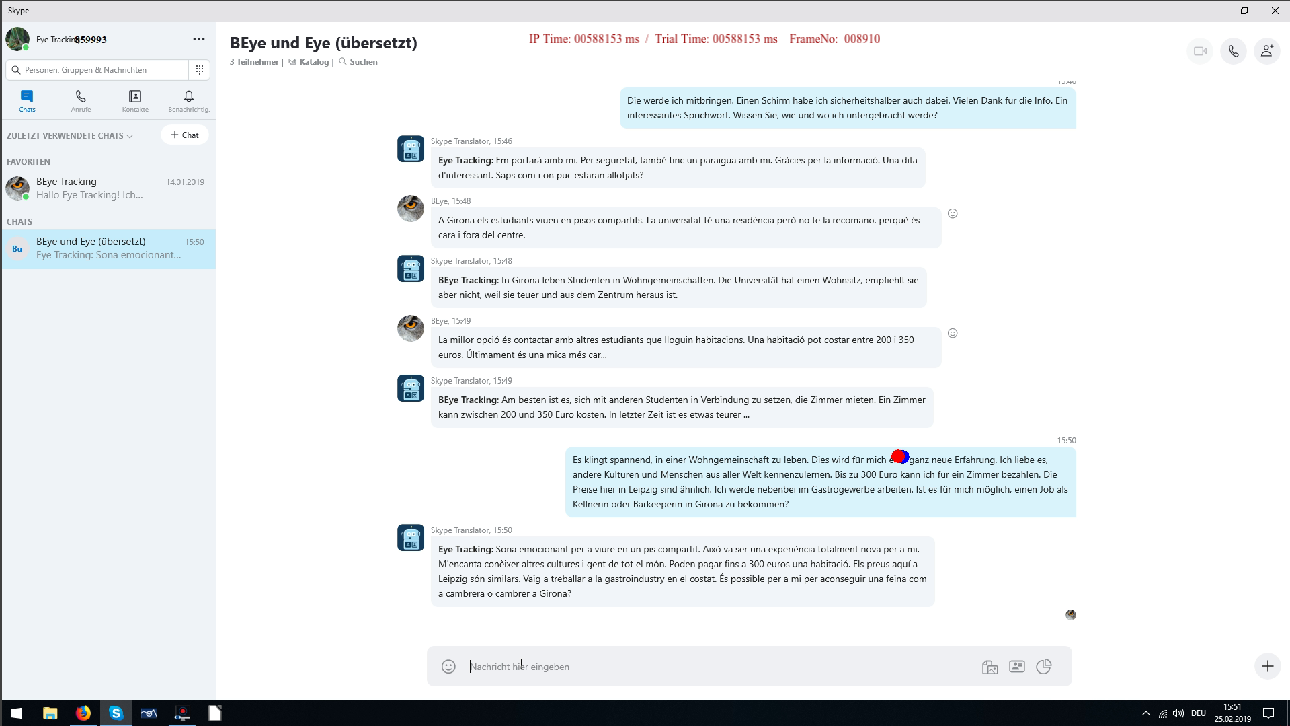
\includegraphics[width=.95\textwidth]{figures/Playback_Image_TN3_Trial_1.png}
    \caption{Example of text boxes in skype. Left-aligned (grey): incoming messages and all MT output. Right-aligned (light blue): original messages of the participant.\label{textboxes}}
\end{figure}


\subsection{Data preparation}
\label{subsec:dataprep}
There are two kinds of analysable data that come from this study. On the one hand, there is the bilingual, authentic linguistic material produced by the participants, the Catalan native speakers and the machine translation of Skype which can be subdivided into four categories: the German and the Catalan original and the machine translated output, respectively. This kind will be spared for further research and publications.

On the other hand, there are the screen captions of the eye tracking sessions. These had to be annotated with dynamic areas of interest as the single text elements in Skype move when a new message is displayed on screen. To allow for a detailed analysis of those four linguistic categories mentioned above, every text box of each session is marked by its own consecutively numbered area of interest (see \figref{textboxes}). Following the language codes proposed by ISO-639-2\footnote{See \url{https://www.bib-bvb.de/web/kkb-online/rda-sprachencode-nach-iso-639}, last accessed on 2020-08-31.}, the following abbreviations were used to label those areas of interest: GerO: German original, GerMT: machine translation into German, CatO: Catalan original, and CatMT: machine translation into Catalan. The entry mask was labelled ``Entry''. Moreover, these five categories allowed for a detailed analysis of the eye tracking data, as it was thus possible to create subsets sorted by participants, by label, by participant and label or other indicators.

The aforementioned 21 eye tracking sessions resulted in the video material of a total duration of 375 minutes, or 18 minutes on average per trial. Taking the interest area count as a measure, the mean of German text messages is 21 (SD~= 9.60, range = 6--48), the mean of machine translated messages into Catalan 20 (SD = 9.79, range = 6--48, the mean of Catalan text messages 27 (SD = 10.85, range = 11--49) and the mean of machine translated messages into German 26 (SD~= 10.66, range = 11--49). A diverging number of original and MT messages can be observed which is explained by the Skype Translator's MT output that was for no obvious reason automatically merged into one text box even if two original messages were written.



%------------------------------------

\section{Results}
\label{sec:Results}


The following observations are based on the categories of interest area labels mentioned above (see Section \ref{subsec:dataprep}). Table~\ref{tab:fixcount} shows the fixation count per area of interest label on aggregate which includes all fixations that fall into the dynamic interest areas of all the participants as described above. The participants are looking more often at the machine translation output than at the original messages regardless of the language. One prominent observation is that both the Catalan and German originals receive less than two thirds the amount of fixations of their respective machine translation equivalent (German original: 2469 to MT into German: 7037 and Catalan original: 3046 to MT into Catalan: 4553).  

\figref{fixDur_AOI} depicts the mean fixation duration per interest area category. The overall mean fixation duration of all fixations falling into the AOI is 314.05ms (SD~= 157.94). The high standard deviation can be attributed to the fact that the participants were mainly resting their eyes at the entry mask when waiting for a response. This is also represented by the highest mean of all categories (348.43ms). The mean of fixations on the German MT output is slightly higher (320ms) than on the original message in German (305ms). The MT output from German into Catalan is fixated longer on average than the original, incoming messages in Catalan (344.93ms to 332.87ms).

%------------------------------------
%\begin{adjustbox}
\begin{table}
\caption{Fixation count per interest area tag}
\label{tab:fixcount}
 \begin{tabular}{lrrrr}
  \lsptoprule
             AOI tag & AOI total & Fix. count & mean & SD \\ 
  \midrule
  GerO  & 433 & 2469 & 6.02 & 13.39 \\
  CatMT  & 429  & 4553 & 11.24 & 17.4\\
  CatO  & 562  & 3046 & 5.61 & 10.20\\
  GerMT  & 551  & 7037 & 13.22 & 16.33\\
  Entry  & 21 & 3964 & 198.20 & 103.93\\
  \lspbottomrule
 \end{tabular}
\end{table}
%\end{adjustbox}
%------------------------------------

% \todo{redo with raw data}
%------------------------------------
\begin{figure}

    \begin{tikzpicture}
        \begin{axis}[
            ybar,
            ylabel = {Mean fixation duration (ms)},
            xlabel = {AOI tag},
            axis lines*=left,
            width  = .7\textwidth,
            height = .3\textheight,
            nodes near coords,
            nodes near coords style = {font=\footnotesize},
            symbolic x coords={GerO,CatMT,CatO,GerMT,Entry},
            xtick=data,
            tick label style={font=\footnotesize},
            x label style={font=\footnotesize},
            y label style={font=\footnotesize},
            nodes near coords,
            ]
            \addplot[black,fill=black] coordinates {
                (GerO,305.24)
                (CatMT,344.93)
                (CatO,332.87)
                (GerMT,320.82)
                (Entry,348.43)
            };
        \end{axis}
    \end{tikzpicture}
    \caption{Mean fixation duration per AOI tag}
    \label{fixDur_AOI}
\end{figure}
%------------------------------------

%------------------------------------

\subsection{Towards an analysis}
\label{subsec:towards_analysis}

As this is just a preliminary look into the collected data of the overall project, at the moment, it is undoubtedly not possible to give a full-range evaluation of the participants' perception on using the Skype Translator to communicate with a counterpart whose mother tongue they do not speak. Nonetheless, a first look into the data set shows that the participants obviously take into account the machine translation output into Catalan despite not being proficient in that language. The differences between fixation count of the original messages and their machine translated counterparts may be taken as a hint for the participants either being at least curious about what their own message is translated to in Catalan or waiting for the Catalan counterpart to respond -- therefore most services display a ``\textit{...currently typing}''-phrase somewhere near the entry mask.
It is possible that by switching between the original and the MT, the participants check on the messages for their integrity or completeness. In addition, even though the fixation count of the Catalan original interest area is equally low to that of the German original compared to the machine translation ones, its fixation duration is higher than the German original and the machine translation into German. To be precise, there are fewer fixations but the ones last longer.
 



%------------------------------------

\section{Conclusion}
\label{sec:conclusion}

The research on computer-mediated communication has been a field of academic interest for a while. Therefore, looking at the bilingual conversations that are mediated by machine translation seems to be a crucial aspect for pointing out how such technology will change the way the users experience these forms of communication. The main task of analysing how conversation partners interact when none of them is proficient in the other's language requires thus special attention to their gaze behaviour, that is, to the way they pay attention to the MT output. Whether this means that they are -- supported by the MT output -- hypothesising about what they are reading or that their attention is simply drawn onto this as it is a new message on the screen has to be profoundly investigated. In this context, an analysis of the regressions that fall into or part from each AOI category seems to be a quite promising approach \citep[cf.][]{eskenazi_regressions_2017}. The collected data thus represents a starting point for evaluating linguistic, cognitive and technological aspects.    


\section*{Abbreviations}

\begin{tabularx}{.5\textwidth}{@{}lQ@{}}
{CatO} & Catalan original\\
{CatMT} & Machine translation into Catalan\\
\end{tabularx}%
\begin{tabularx}{.5\textwidth}{@{}lQ@{}}
{GerO} & German original\\
{GerMT} & Machine translation into German
\end{tabularx}

\section*{Acknowledgements}
I am grateful to our institute's student assistant Tim Feldmüller, who took care of preparing most of the collected research data.

{\sloppy\printbibliography[heading=subbibliography,notkeyword=this]}
\end{document}
